\documentclass[../main.tex]{subfiles}

\begin{document}

\subsection{Simulación de los circuitos RC y RL}
El primer paso a llevar a cabo en la implementación de las simulaciones de los circuitos RC y RL, será plantear un algoritmo que nos permita generar los datos correspondientes a cada una de las magnitudes físicas de ambos circuitos.\\ 

\subsubsection{Etapas del proceso}
Comenzamos entonces identificando cuáles son las etapas en las que podemos dividir el proceso de llevar a cabo una simulación:

\begin{itemize}
    \item En primer lugar tenemos la etapa de \textit{stop} en la que, como su propio nombre indica, el sistema se encuentra totalmente en reposo, pausando así los subprocesos de generación y representación de resultados. Por defecto, esta etapa será activada cada vez que se cree una nueva instancia de cualquiera de los dos circuitos. \\

    Dado que el proceso de la simulación se encuentra pausado en esta fase, para pasar a cualquiera de las otras (ver siguientes) el usuario debe de forzar al sistema utilizando el interfaz de usuario de la aplicación.

    \item La segunda etapa a destacar y que podriamos considerar como la principal, consta de un subproceso cíclico en el que se lleva a cabo la generación, el procesamiento y el almacenamiento de los datos; y paralelamente, su representación. Esta etapa estará activa siempre y cuando la simulación no haya finalizado por alguna de las siguientes causas: el circuito a simular no haya alcanzado su estado de equilibrio y por lo tanto, no tiene sentido seguir generando resultados; se haya cumplido alguna de las restricciones impuestas por el usuario; o bien, la simulación haya sido reiniciada manualmente. Este último caso es algo especial, el cuál veremos en el siguiente punto. \\

    A esta etapa del proceso de la simulación la denominaremos etapa activa o \textit{running}.

    \item Como hemos comentado anteriormente, es posible reiniciar la simulación de forma manual, iniciando entonces la etapa de \textit{reload} o reinicio. En ella se hace una limpieza de todos los resultados que se han ido generando previamente y justo después, se vuelve a iniciar la simulación del último circuito establecido, volviendo así a la etapa de \textit{running}. 

    \item Por último, tenemos el subproceso de cambiar de valor un componente del circuito. Aunque esta no será considerada como una etapa más del proceso sino más bien como un paso intermedio entre la  
    simulación de dos circuitos diferentes ya que en este no se actúa directamente sobre los resultados de la simulación actual, cabe destacar que al igual que al igual que la etapa de \textit{reload}, se trata de un subproceso donde la finalización de este no depende del usuario, sino del propio flujo del sistema. 
    
   
\end{itemize}

Para comprender mejor el funcionamiento global de la simulación, se ha elaborado el diagrama de la figura \ref{fig::diagrama-algoritmo}, en el que se puede ver con mayor detalle la interacción entre los diferentes subprocesos.\\


\begin{figure}[!h]
    \centering
    \includegraphics[width=\textwidth]{images/diagrama-algoritmo.png}
    \caption{Representación abstracta la aplicación. Las flechas en \textit{rojo} indican las acciones que el usuario puede tomar sobre la aplicación; en \textit{negro} las acciones que toma el sistema por su cuenta. }
    \label{fig::diagrama-algoritmo}
\end{figure}

 A continuación presentamos los aspectos más importantes de las simulaciones, en los que trataremos conceptos como \textit{ventana de datos} o \textit{condiciones de parada}.


\subsubsection{Generación de datos}
Que el sistema se encuentre en las etapas de \textit{stop} o \textit{reload} depende más de las acciones que tome el usuario de la aplicación que del propio flujo del proceso, por lo que nos centraremos en la etapa activa para la generación de datos en tiempo real. Nos apoyeremos entonces en el método \textit{componentDidMount} del componente de la simulación, que como ya sabemos, solamente se ejecuta una vez durante la vida de un componente (concretamente durante su creación). \\

Aprovechando la capacidad de JavaScript para crear funciones privadas en el cuerpo de otros métodos y funciones, crearemos la instancia de una nueva función local y asíncrona dentro del procedimiento \textit{componentDidMount}, la cuál se ejecutará repetitivamente cada cierto tiempo, como por ejemplo cada 150 milisegundos (a estas funciones también se le conocen como \textit{setInterval}). La elección del valor de este intervalo se toma en base a la velocidad de generación de los datos que queramos. Si este es muy grande, el tiempo de espera entre la producción de dos valores crece demasiado, ralentizando así la representación de los mismos; pero si es muy pequeño, la cantidad de información generada podría llegar a ser demasiado grande, pudiendo llegar a colapsar la propia aplicación. Frente a las alternativas que presenta este dilema nos quedamos con la segunda opción, pues podemos hacer uso de una \textit{ventana de datos} de longitud fija para almacenar los resultados.

Por cada magnitud física a representar, utilizaremos una ventana de datos diferente. Se trata de una lista de longitud no variable sobre la que debemos de controlar la inserción de nuevos resultados. Cuando el número de datos de la ventana es inferior a su longitud no existe ningún problema, pues podemos ir añadiendo otros  nuevos al final de la misma y mantener así el orden de producción (figura \ref{fig::ventana_datos_1}). Sin embargo, si excedemos el límite, lo que haremos será eliminar el de mayor antigüedad, desplazando el resto una posición hacia la izquierda (\textit{shift}) y obteniendo así un hueco libre para añadir nueva información (figura \ref{fig::ventana_datos_2}). El objetivo de esto no es otro que mantener el orden de llegada para que la representación de los resultados sea lo más cómoda posible. \\


\begin{figure}[!h]
    \centering
    \includegraphics[width=0.9\textwidth]{images/ventana_datos_1.png}
    \caption{Cada que generamos un nuevo resultado y aún queda espacio libre, este se añade al final de la lista, respetando así el orden en el que fueron generados.}
    \label{fig::ventana_datos_1}
\end{figure}

\begin{figure}[!h]
    \centering
    \includegraphics[width=\textwidth]{images/ventana_datos_2.png}
    \caption{Cuando ya no queda hueco libre en la ventana de datos, realizamos un \textit{shift} de esta lista, dejando así espacio libre para la insercion de nuevos resultados.}
    \label{fig::ventana_datos_2}
\end{figure}

Además, las funciones del tipo \textit{setInterval} retornan un valor identificativo que hacen referencia al temporizador de la función. Este será utilizado por el componente asociado al simulador en su etapa de destrucción para eliminar la llamada reiterativa de este proceso. Y aunque realmente esta limpieza no es necesaria (ya que solamente tendremos una función de este tipo ejecutándose al mismo tiempo), si que es de buena práctica llevarla a cabo, pues si el número de funciones \textit{setInterval} utilizadas es mayor puede causar problemas de rendimiento en la aplicación si no se toman este tipo de medidas.\\

\subsubsection{Tiempo absoluto y tiempo relativo de la simulación}
Por otro lado, para garantizar la correcta visualización de los datos correspondientes a cada una de las magnitudes físicas en las gráficas, tenemos que considerar dos valores de tiempo diferentes, los cuales vamos a denominar como \textit{tiempo absoluto} y \textit{tiempo relativo} de la simulación.\\

El primero de ellos, al que hemos llamado como \textit{tiempo absoluto}, será de utilidad para la representación de cada una de las magnitudes en un mismo eje. Como es lógico, esta variable de tiempo se verá incrementada a medida que se van obteniendo nuevos resultados de la simulación, tomando solamente valor nulo cuando se cree por primera vez la instancia del circuito o bien, la simulación sea reiniciada manualmente por el usuario en la etapa de \textit{reload}. 

Sin embargo, para calcular los resultados de cada una de las magnitudes físicas que describen el circuito en un instante de tiempo determinado, utilizaremos el \textit{tiempo relativo} de la simulación, el cuál tomará siempre valor cero cada vez que alguno de los componentes del circuito sea alterado y que se verá incrementado a la par que lo hace la variable de \textit{tiempo absoluto}.\\

De esta manera, utilizando una variable para el tiempo relativo podremos obtener los resultados de la simulación utilizando las expresiones del modelado en un instante de tiempo determinado y, al mismo tiempo, dicho valor lo almacenaremos con el valor de la variable de tiempo absoluto de la simuluación. Esto permite visualizar en un mismo eje los resultados obtenidos de varias simulaciones, facilitando así la comparación entre ellos. Por ejemplo, en la figura \ref{fig::tiempos_simulacion} podemos observar con más detalle el uso de cada una de estas variables durante la simulación de un circuito RC, en el que vemos la evolución de la carga de un condensador cuando pasamos de una fuente de $12V$ a una de $6V$.\\




 \begin{figure}[!h]
        \centering
                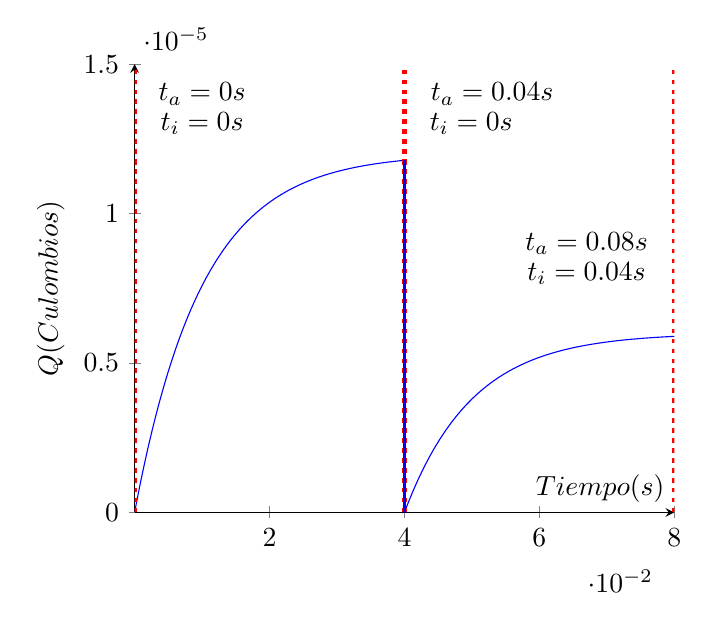
\begin{tikzpicture}
            \begin{axis}[
                axis y line = left,
                axis x line = middle,
                xmin=0,
                ymin=0, 
                xlabel = \(Tiempo (s)\),
                ylabel = {\(Q (Culombios)\)},
            ]
            %Below the red parabola is defined
            \addplot [
                domain=0:0.04, 
                samples=1000, 
                color=blue,
            ]
            {0.000012*(1-exp(-x/0.01))};
             
            \addplot [
                domain=0:0.08, 
                samples=100, 
                color=blue,
            ]
            {0.000006*(1-exp((-x + 0.04)/0.01))};

            %% Vertical line
            \addplot[ultra thick, dotted, samples=50, smooth, domain=0:0.08, red] coordinates {(0.04,0)(0.04, 0.000015)};
            
            \addplot[thick, samples=50, smooth, domain=0:0.08, blue] coordinates {(0.04,0)(0.04, 0.00001178)};

            \node[inner sep=1pt,] (0.04) at (0.0499,0.000013) {$t_i = 0s$};
            \node[inner sep=1pt,] (0.04) at (0.053, 0.000014) {$t_a = 0.04s$};


            %% Vertical left line
            \addplot[ultra thick, dotted, samples=50, smooth, domain=0:0.08, red] coordinates {(0.08,0)(0.08, 0.000015)};
            \node[inner sep=1pt,] (0.08) at (0.067, 0.000008) {$t_i = 0.04s$};
            \node[inner sep=1pt,] (0.08) at (0.067, 0.000009) {$t_a = 0.08s$};

            %% Vertical left line
            \addplot[ultra thick, dotted, samples=50, smooth, domain=0:0.08, red] coordinates {(0,0)(0, 0.000015)};
            \node[inner sep=1pt,] (0) at (0.01, 0.000013) {$t_i = 0s$};
            \node[inner sep=1pt,] (0) at (0.01, 0.000014) {$t_a = 0s$};
            
        
        \end{axis}
        \end{tikzpicture}

        \caption{Ejemplo de cómo se vería la evolución de la carga de un condensador en una simulación del circuito RC, donde se aprecian los valores que toman tanto el \textit{tiempo absoluto} ($t_a$) como el \textit{tiempo relativo} ($t_i$) cuando pasamos de una fuente de $12V$ a una de $6V$.}

        \label{fig::tiempos_simulacion}
    \end{figure}


\subsubsection{Condiciones de parada y escala de tiempo}
Otro aspecto importante a tener en cuenta es la finalización de las simulaciones de los circuitos RC y RL. Por defecto, una simulación de cualquier circuito se dará por terminada cuando este alcance su estado de equilibrio; es decir, cuando las magnitudes físicas estudiadas tomen su valor máximo o mínimo dependiendo de si estas son crecientes o decrecientes en el tiempo. Sin embargo, lo más probable es que en ocasiones no sea necesario recopilar información sobre la simulación completa, sino que basta con obtener datos hasta que se cumpla cierta condición. Estas condiciones son las siguientes:\\

\begin{itemize}
    \item En el caso del circuito RC, el cuál lo estudiamos según la evolución de la carga del condensador, tomaremos como restricciones el valor o porcentaje máximo de carga del condensador.

    \item En el caso del circuito RL, la magnitud física que tendremos en cuenta para finalizar la simulación será la intensidad de corriente, ya sea dando su valor en \textit{amperios} o el tanto por ciento de dicha magnitud.

    \item Además, en ambos casos se implementará la posibilidad de simular los circuitos durante un tiempo determinado.
    
\end{itemize}

Sin embargo, nos podemos encontrar con el problema presentado en la figura \ref{fig::condicion-parada-1}, en la que se puede ver que la precisión de los resultados obtenidos no es muy buena. Nos encontramos entonces un margen de error entre los resultados esperados (líneas verticales y discontinuas) y los resultados obtenidos en la simulación (final de las líneas naranja y azul), cuya diferencia mostrada de color rojo es el error cometido. Para reducir este error lo que se propone es implementar un modificador de la escala de tiempo, el cuál permita al usuario establecer cuál será el intervalo de tiempo que transcurre en la generación entre cada par de datos, con el objetivo de minimizar lo máximo posible el margen de error cometido.

Esto cuenta con un inconveniente y es que, cuanto menor sea la escala de tiempo utilizada mayor será el tiempo empleado en la generación de datos y por consiguiente, mayor tiempo se necesitará en mostrar los resultados. Esto dependerá del usuario de la aplicación en utilizar una escala de tiempo que se ajuste a sus necesidades.\\

En la figura \ref{fig::condiciones-de-parada} se puede ver con más detalle cómo el error cometido se reduce al disminuir la escala de tiempo para un mismo circuito RC, utilizando como condición de parada que el porcentaje de carga no sobrepase el 63.08\% de la carga máxima.\\ 


\begin{figure}[!h]
    \centering
    \subfloat[Escala de tiempo: 10s]{
        \label{fig::condicion-parada-1}
        \includegraphics[width=0.45\textwidth]{images/carga-condicion-3.PNG}
    }
    \quad
    \subfloat[Escala de tiempo: 1s]{
        \label{fig::condicion-parada-2}
        \includegraphics[width=0.45\textwidth]{images/carga-condicion-2.PNG}
    }


    \subfloat[Escala de tiempo: 1ms]{
        \label{fig::condicion-parada-3}
        \includegraphics[width=0.45\textwidth]{images/carga-condicion-1.PNG}
    }
    \caption{Simulación de la carga del condensador bajo la condición de parada de que esta sea menor que el 63.08\% de su capacidad. En \textit{azul} se muestran los resultados obtenidos en estado de almacenamiento de energía; en \textit{naranja} en estado de disipación de energía.}

    \label{fig::condiciones-de-parada}
\end{figure}






\subsection{Comparación de resultados}
Por último, para comprobar que efectivamente los resultados que se están generando en nuestra aplicación coinciden o se aproximan lo suficiente a los reales, deberemos de realizar una serie de pruebas que nos permitan comparar ambos resultados. Para ello, se ha elaborado un script de \textit{python} utilizando las librerías de \textit{numpy} \cite{numpy} y \textit{matplotlib} \cite{matplotlib}, el cuál se encarga de generar una imagen con los resultados de una simulación cualquiera en la que se muestra información  adicional de la misma, como la carga o intensidad de corriente final que se ha alcanzado en cada uno de los estados del circuito o el tiempo empleado en realizar dicha simulación.\\ 


Para los casos de prueba, utilizaremos un circuito RC con una resistencia de $3\Omega$, una fuente de $5V$ y un condensador con una capacidad de $10F$. Por otro lado, para las pruebas del circuito RL usaremos una resistencia de $15\Omega$, una fuente con un valor de $20V$ y una bobina de $5H$ de inductancia. En el caso de la escala de tiempo a utilizar, se tomará aquella que genere resultados con el menor índice de error posible (escalas muy pequeñas). Además, el número de pruebas se han limitado a cuatro, en las cuáles se probarán las simulaciones completas de los circuitos, así como estos mismos bajo ciertas condiciones.\\



\subsubsection{Caso de prueba 1: carga y descarga de un condensador}

El primer caso de prueba simularemos el circuito RC, sin condiciones de parada y utilizando una escala de tiempo de $1s$. Si realizamos la simulación en la aplicación, obtenemos los resultados que se muestran en la figuras \ref{fig::cp1-app} y \ref{fig::cp1.1-app}. \\

\begin{figure}[!h]
    \centering
    \includegraphics[width=0.8\textwidth]{images/cp1-app.PNG}
    \caption{Caso de prueba 1: resultados de la aplicación. Estado de carga.}
    \label{fig::cp1-app}
\end{figure}

\begin{figure}[!h]
    \centering
    \includegraphics[width=0.8\textwidth]{images/cp1.1-app.PNG}
    \caption{Caso de prueba 1: resultados de la aplicación. Estado de descarga.}
    \label{fig::cp1.1-app}
\end{figure}


El estado de equilibrio del circuito se alcanza a los $150$ segundos. luego, si simulamos durante ese tiempo en el script que hemos desarrollado, obtenemos los siguientes resultados (figura \ref{fig::cp1.1-py}), en el que comprobamos que efectivamente la carga máxima alcanzada es de 50 culombios.\\

\begin{figure}[!h]
    \centering
    \includegraphics[width=0.8\textwidth]{images/cp1-py.png}
    \caption{Caso de prueba 1: resultados del script. }
    \label{fig::cp1.1-py}
\end{figure}

\subsubsection{Caso de prueba 2: carga y descarga de un condensador (con restricciones)}
Para este segundo caso de prueba, utilizaremos como restricción que el porcentaje de carga del condensador no sea superior al $40\%$. Los resultados obtenidos en la aplicación son los siguientes mostrados en las figuras \ref{fig::cp2-app} y \ref{fig::cp2.1-app}; además, volvemos a utilizar los segundos como escala de tiempo.\\ 

\begin{figure}[!h]
    \centering
    \includegraphics[width=0.8\textwidth]{images/cp2-app.PNG}
    \caption{Caso de prueba 2: resultados de la aplicación. Estado de carga.}
    \label{fig::cp2-app}
\end{figure}

\begin{figure}[!h]
    \centering
    \includegraphics[width=0.8\textwidth]{images/cp2.1-app.PNG}
    \caption{Caso de prueba 2: resultados de la aplicación. Estado de descarga.}
    \label{fig::cp2.1-app}
\end{figure}

Según los resultados de la aplicación, el valor de la carga cuando la simulación finaliza a los $15$ segundos es ligeramente inferior a $20C$, el cuál coincide con los resultados obtenidos al utilizar el \textit{script} de \textit{python}, dónde obtenemos que la carga está sobre los $19.67C$. Sin embargo, en la información adicional que nos proporciona la imagen generada (figura \ref{fig::cp2.1-py}) se detalla que la carga es de $20C$ y que esta se alcanza a los $15.32$ segundos; y aunque los resultados se asemejan bastante, estos no llegan a coincidir, así que para obtener datos más precisos deberemos de reducir la escala de tiempo, tal y como ya se comentó anteriormente. 

\begin{figure}[!h]
    \centering
    \includegraphics[width=0.8\textwidth]{images/cp2-py.png}
    \caption{Caso de prueba 2: resultados del script. }
    \label{fig::cp2.1-py}
\end{figure}

\subsubsection{Caso de prueba 3: carga y descarga de un inductor}
Pasamos entonces al tercer caso de prueba, donde simularemos un circuito RL con los parámetros indicados anteriormente, con una escala de tiempo en \textit{milisegundos}. Mediante la aplicación, obtenemos los resultados que se muestran en las figuras \ref{fig::cp3-app} y \ref{fig::cp3.1-app}.

\begin{figure}[!h]
    \centering
    \includegraphics[width=0.8\textwidth]{images/cp3-1.PNG}
    \caption{Caso de prueba 3: resultados de la aplicación. Estado de carga.}
    \label{fig::cp3-app}
\end{figure}

\begin{figure}[!h]
    \centering
    \includegraphics[width=0.8\textwidth]{images/cp3-1.1.PNG}
    \caption{Caso de prueba 3: resultados de la aplicación. Estado de descarga.}
    \label{fig::cp3.1-app}
\end{figure}

\begin{figure}[!h]
    \centering
    \includegraphics[width=0.8\textwidth]{images/cp3-py.png}
    \caption{Caso de prueba 3: resultados del script. }
    \label{fig::cp3-py}
\end{figure}




\subsubsection{Caso de prueba 4: carga y descarga de un inductor (con restricciones)}










\end{document}